\documentclass[12pt,a4paper]{article}
\usepackage[utf8]{inputenc}
\usepackage{amsmath}
\usepackage{amsfonts}
\usepackage{amssymb}
\usepackage{graphicx}
\usepackage{tikz}
\usetikzlibrary{automata,positioning,arrows.meta,shapes}
\usepackage{geometry}
\usepackage{listings}
\usepackage{xcolor}
\usepackage{fancyhdr}
\usepackage{hyperref}
\usepackage{tabularx}

\geometry{margin=1in}
\pagestyle{fancy}
\fancyhf{}
\rhead{Lexical Analysis Theory}
\lhead{Assignment 01 v1}
\cfoot{\thepage}

% Code listing style
\lstset{
    language=C,
    basicstyle=\ttfamily\small,
    keywordstyle=\color{blue},
    commentstyle=\color{green!60!black},
    stringstyle=\color{red},
    numbers=left,
    numberstyle=\tiny,
    breaklines=true,
    frame=single,
    tabsize=4
}

\title{\textbf{Lexical Analysis: Theory and Implementation}\\
\large{Assignment 01 Version 1 - Detailed Theoretical Documentation}}
\author{Compiler Design Laboratory}
\date{\today}

\begin{document}

\maketitle

\tableofcontents
\newpage

\section{Introduction}

This document provides comprehensive theoretical documentation for the lexical analyzer implementation in Assignment 01 Version 1. It covers the fundamental concepts of compiler design, finite state automata, regular expressions, and the equivalence between theoretical concepts and practical code implementation.

\subsection{Purpose}
The lexical analyzer (or lexer) is the first phase of a compiler that converts a stream of characters into a stream of tokens. It serves as the interface between the source program text and the subsequent compiler phases.

\subsection{Scope}
This implementation recognizes:
\begin{itemize}
    \item Arithmetic Operators: \texttt{+}, \texttt{-}, \texttt{*}, \texttt{/}, \texttt{\%}, \texttt{++}, \texttt{--}
    \item Relational Operators: \texttt{<}, \texttt{>}, \texttt{<=}, \texttt{>=}, \texttt{==}, \texttt{!=}
    \item Logical Operators: \texttt{\&\&}, \texttt{||}, \texttt{!}
    \item Bitwise Operators: \texttt{\&}, \texttt{|}, \texttt{\^{}}, \texttt{\~{}}, \texttt{<<}, \texttt{>>}
    \item Assignment Operators: \texttt{=}, \texttt{+=}, \texttt{-=}, \texttt{*=}, \texttt{/=}, \texttt{\%=}, \texttt{\&=}, \texttt{|=}, \texttt{\^{}=}, \texttt{<<=}, \texttt{>>=}
    \item Keywords: \texttt{int}, \texttt{float}, \texttt{char}, \texttt{for}, \texttt{while}, \texttt{if}, \texttt{else}
    \item Identifiers and Integer Constants
    \item Delimiters: Parentheses and Braces
\end{itemize}

\section{Theoretical Foundation}

\subsection{Compiler Architecture}

The compiler is organized into several phases, with lexical analysis being the first:

\begin{figure}[h!]
\centering
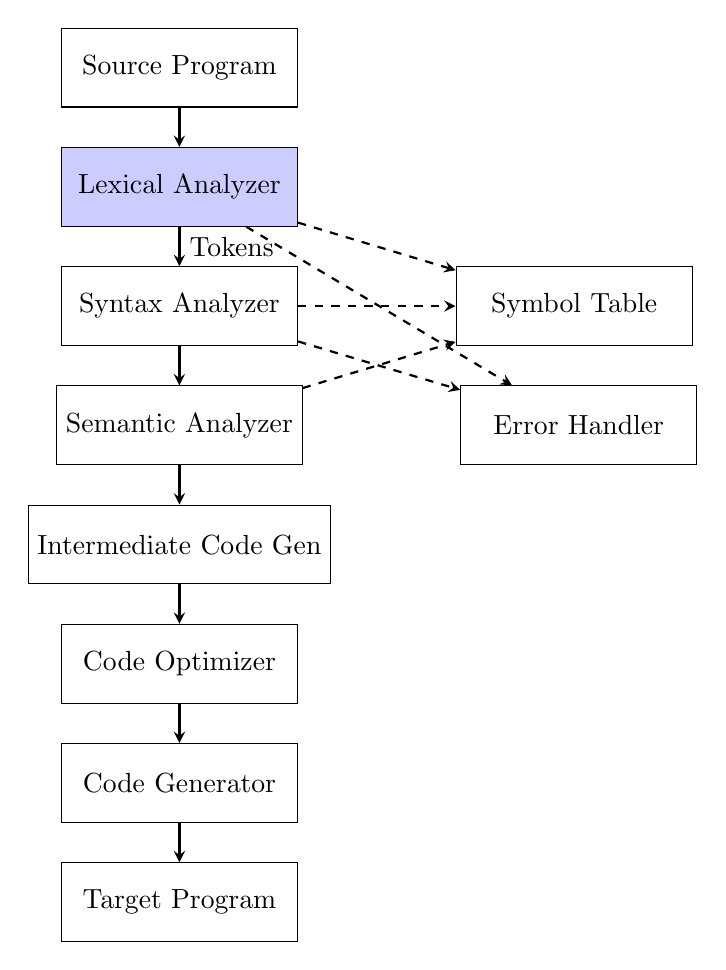
\begin{tikzpicture}[
    box/.style={rectangle, draw, minimum width=3cm, minimum height=1cm, text centered},
    arrow/.style={->, >=stealth, thick}
]
    \node[box] (source) {Source Program};
    \node[box, below=0.5cm of source, fill=blue!20] (lex) {Lexical Analyzer};
    \node[box, below=0.5cm of lex] (syn) {Syntax Analyzer};
    \node[box, below=0.5cm of syn] (sem) {Semantic Analyzer};
    \node[box, below=0.5cm of sem] (icg) {Intermediate Code Gen};
    \node[box, below=0.5cm of icg] (opt) {Code Optimizer};
    \node[box, below=0.5cm of opt] (cg) {Code Generator};
    \node[box, below=0.5cm of cg] (target) {Target Program};
    
    \node[box, right=2cm of syn] (st) {Symbol Table};
    \node[box, right=2cm of sem] (eh) {Error Handler};
    
    \draw[arrow] (source) -- (lex);
    \draw[arrow] (lex) -- node[right] {Tokens} (syn);
    \draw[arrow] (syn) -- (sem);
    \draw[arrow] (sem) -- (icg);
    \draw[arrow] (icg) -- (opt);
    \draw[arrow] (opt) -- (cg);
    \draw[arrow] (cg) -- (target);
    
    \draw[arrow, dashed] (lex) -- (st);
    \draw[arrow, dashed] (syn) -- (st);
    \draw[arrow, dashed] (sem) -- (st);
    \draw[arrow, dashed] (lex) -- (eh);
    \draw[arrow, dashed] (syn) -- (eh);
\end{tikzpicture}
\caption{Compiler Architecture with Lexical Analyzer Highlighted}
\end{figure}

\subsection{Role of Lexical Analyzer}

The lexical analyzer has several key responsibilities:

\begin{enumerate}
    \item \textbf{Tokenization}: Convert character stream into token stream
    \item \textbf{Whitespace Removal}: Skip spaces, tabs, and newlines
    \item \textbf{Comment Removal}: Skip comments (if implemented)
    \item \textbf{Line Tracking}: Maintain line numbers for error reporting
    \item \textbf{Error Detection}: Identify and report invalid tokens
    \item \textbf{Symbol Table Interaction}: Insert identifiers into symbol table
\end{enumerate}

\subsection{Regular Expressions}

Token patterns are specified using regular expressions:

\begin{table}[h!]
\centering
\begin{tabular}{|l|l|l|}
\hline
\textbf{Token Type} & \textbf{Regular Expression} & \textbf{Examples} \\
\hline
Keyword & \texttt{int | float | char | for | while | if | else} & \texttt{int}, \texttt{while} \\
Identifier & \texttt{[a-zA-Z\_][a-zA-Z0-9\_]*} & \texttt{x}, \texttt{count}, \texttt{\_temp} \\
Integer & \texttt{[0-9]+} & \texttt{0}, \texttt{123}, \texttt{9999} \\
Whitespace & \texttt{[ \textbackslash t\textbackslash n]+} & (space), (tab), (newline) \\
\hline
\end{tabular}
\caption{Token Pattern Specifications}
\end{table}

\section{Finite State Automata}

\subsection{Mathematical Definition}

A Finite State Automaton (FSA) is formally defined as a 5-tuple:
\[ M = (Q, \Sigma, \delta, q_0, F) \]

Where:
\begin{itemize}
    \item $Q$ is a finite set of states
    \item $\Sigma$ is the input alphabet (set of characters)
    \item $\delta: Q \times \Sigma \rightarrow Q$ is the transition function
    \item $q_0 \in Q$ is the start state
    \item $F \subseteq Q$ is the set of accepting (final) states
\end{itemize}

\subsection{FSA for Identifier Recognition}

\begin{figure}[h!]
\centering
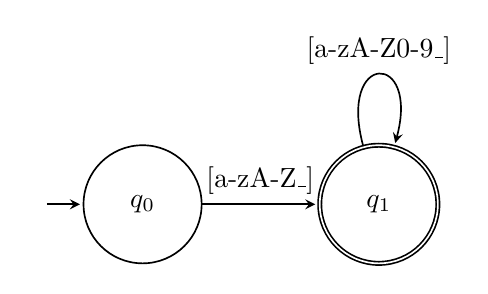
\begin{tikzpicture}[
    > = stealth,
    shorten > = 1pt,
    auto,
    node distance = 3cm,
    semithick,
    initial text=,
    state/.style={circle, draw, minimum size=1.5cm}
]
    \node[state, initial] (q0) {$q_0$};
    \node[state, accepting, right of=q0] (q1) {$q_1$};
    
    \path[->]
        (q0) edge node {[a-zA-Z\_]} (q1)
        (q1) edge [loop above] node {[a-zA-Z0-9\_]} (q1);
\end{tikzpicture}
\caption{FSA for Identifier Recognition}
\end{figure}

\textbf{Formal Specification:}
\begin{align*}
Q &= \{q_0, q_1\} \\
\Sigma &= \{\text{a-z, A-Z, 0-9, \_}\} \\
q_0 &= q_0 \\
F &= \{q_1\} \\
\delta(q_0, c) &= \begin{cases}
    q_1 & \text{if } c \in [a\text{-}zA\text{-}Z\_] \\
    \text{error} & \text{otherwise}
\end{cases} \\
\delta(q_1, c) &= \begin{cases}
    q_1 & \text{if } c \in [a\text{-}zA\text{-}Z0\text{-}9\_] \\
    \text{accept} & \text{otherwise (retract)}
\end{cases}
\end{align*}

\subsection{FSA for Integer Recognition}

\begin{figure}[h!]
\centering
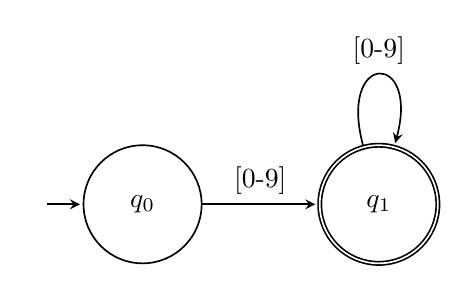
\begin{tikzpicture}[
    > = stealth,
    shorten > = 1pt,
    auto,
    node distance = 3cm,
    semithick,
    initial text=,
    state/.style={circle, draw, minimum size=1.5cm}
]
    \node[state, initial] (q0) {$q_0$};
    \node[state, accepting, right of=q0] (q1) {$q_1$};
    
    \path[->]
        (q0) edge node {[0-9]} (q1)
        (q1) edge [loop above] node {[0-9]} (q1);
\end{tikzpicture}
\caption{FSA for Integer Recognition}
\end{figure}

\subsection{FSA for Plus Operator (+, ++, +=)}

\begin{figure}[h!]
\centering
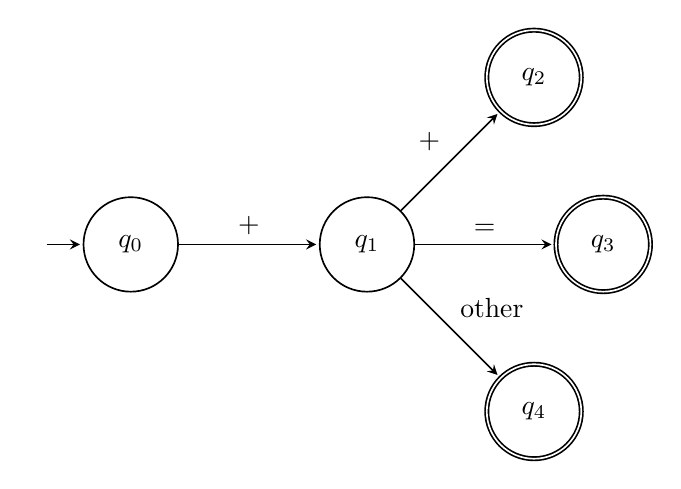
\begin{tikzpicture}[
    > = stealth,
    shorten > = 1pt,
    auto,
    node distance = 3cm,
    semithick,
    initial text=,
    state/.style={circle, draw, minimum size=1.2cm}
]
    \node[state, initial] (q0) {$q_0$};
    \node[state, right of=q0] (q1) {$q_1$};
    \node[state, accepting, above right of=q1] (q2) {$q_2$};
    \node[state, accepting, right of=q1] (q3) {$q_3$};
    \node[state, accepting, below right of=q1] (q4) {$q_4$};
    
    \path[->]
        (q0) edge node {+} (q1)
        (q1) edge node {+} (q2)
        (q1) edge node {=} (q3)
        (q1) edge node {other} (q4);
\end{tikzpicture}
\caption{FSA for Plus Operator Variations}
\end{figure}

Where:
\begin{itemize}
    \item $q_2$ accepts \texttt{++} (arithmetic operator)
    \item $q_3$ accepts \texttt{+=} (assignment operator)
    \item $q_4$ accepts \texttt{+} (arithmetic operator, with input retraction)
\end{itemize}

\subsection{FSA for Shift Operators (<<, <<=, <, <=)}

\begin{figure}[h!]
\centering
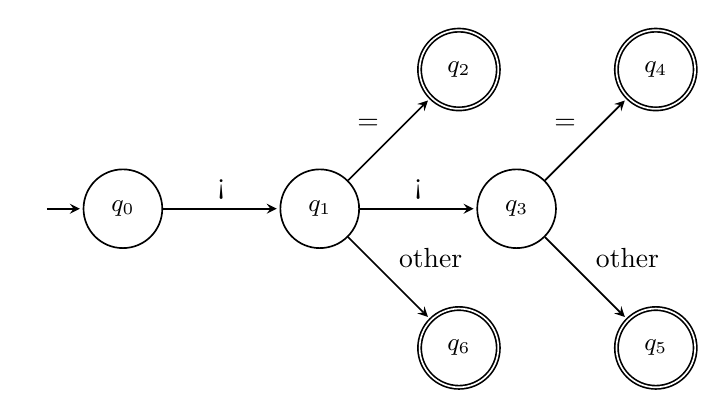
\begin{tikzpicture}[
    > = stealth,
    shorten > = 1pt,
    auto,
    node distance = 2.5cm,
    semithick,
    initial text=,
    state/.style={circle, draw, minimum size=1cm, font=\small}
]
    \node[state, initial] (q0) {$q_0$};
    \node[state, right of=q0] (q1) {$q_1$};
    \node[state, accepting, above right of=q1] (q2) {$q_2$};
    \node[state, right of=q1] (q3) {$q_3$};
    \node[state, accepting, above right of=q3] (q4) {$q_4$};
    \node[state, accepting, below right of=q3] (q5) {$q_5$};
    \node[state, accepting, below right of=q1] (q6) {$q_6$};
    
    \path[->]
        (q0) edge node {<} (q1)
        (q1) edge node {=} (q2)
        (q1) edge node {<} (q3)
        (q3) edge node {=} (q4)
        (q3) edge node {other} (q5)
        (q1) edge node {other} (q6);
\end{tikzpicture}
\caption{FSA for Left Shift and Less Than Operators}
\end{figure}

Accepting states correspond to:
\begin{itemize}
    \item $q_2$: \texttt{<=} (relational operator)
    \item $q_4$: \texttt{<<=} (assignment operator)
    \item $q_5$: \texttt{<<} (bitwise operator, with retraction)
    \item $q_6$: \texttt{<} (relational operator, with retraction)
\end{itemize}

\section{Token Recognition Algorithms}

\subsection{General Token Recognition}

The lexical analyzer uses the following algorithm:

\begin{lstlisting}
TokenType yylex(void) {
    State current_state = STATE_START;
    buffer_index = 0;
    
    while (1) {
        char c = get_char();
        
        // Skip whitespace
        while (c == ' ' || c == '\t' || c == '\n') {
            if (c == '\n') yylineno++;
            c = get_char();
        }
        
        if (c == EOF)
            return TOKEN_EOF;
            
        // State transitions based on current state
        switch (current_state) {
            case STATE_START:
                // Determine token type
                break;
            // ... other states
        }
    }
}
\end{lstlisting}

\subsection{Keyword vs Identifier Disambiguation}

After recognizing an identifier pattern, the lexer checks if it's a keyword:

\begin{lstlisting}
int is_keyword(const char *str) {
    const char *keywords[] = {
        "int", "float", "char", 
        "for", "while", "if", "else"
    };
    int num_keywords = 7;
    
    for (int i = 0; i < num_keywords; i++) {
        if (strcmp(str, keywords[i]) == 0)
            return 1;
    }
    return 0;
}

// Usage in lexer
if (is_keyword(yytext))
    return TOKEN_KEYWORD;
else
    return TOKEN_IDENTIFIER;
\end{lstlisting}

\subsection{Multi-Character Operator Recognition}

Complex operators require lookahead:

\begin{lstlisting}
// Recognize '<' variants
case '<':
    add_to_buffer('<');
    c = get_char();
    
    if (c == '=') {
        add_to_buffer('=');
        return TOKEN_RELATIONAL_OP;  // <=
    }
    else if (c == '<') {
        add_to_buffer('<');
        c = get_char();
        if (c == '=') {
            add_to_buffer('=');
            return TOKEN_ASSIGNMENT_OP;  // <<=
        }
        else {
            unget_char(c);
            return TOKEN_BITWISE_OP;  // <<
        }
    }
    else {
        unget_char(c);
        return TOKEN_RELATIONAL_OP;  // <
    }
\end{lstlisting}

\section{Implementation Details}

\subsection{Global Variables (lex Conventions)}

The implementation follows standard lex/yacc conventions:

\begin{lstlisting}
char *yytext = NULL;    // Points to current token
int yyleng = 0;         // Length of current token
int yylineno = 1;       // Current line number
FILE *yyin = NULL;      // Input file pointer
\end{lstlisting}

\subsection{Token Structure}

Tokens are represented by an enumeration:

\begin{lstlisting}
typedef enum {
    TOKEN_EOF = 0,
    TOKEN_IDENTIFIER,
    TOKEN_INTEGER,
    TOKEN_KEYWORD,
    TOKEN_ARITHMETIC_OP,
    TOKEN_RELATIONAL_OP,
    TOKEN_LOGICAL_OP,
    TOKEN_BITWISE_OP,
    TOKEN_ASSIGNMENT_OP,
    TOKEN_LPAREN,
    TOKEN_RPAREN,
    TOKEN_LBRACE,
    TOKEN_RBRACE,
    TOKEN_SEMICOLON,
    TOKEN_ERROR
} TokenType;
\end{lstlisting}

\subsection{Buffer Management}

\begin{lstlisting}
#define MAX_TOKEN_LENGTH 256
char token_buffer[MAX_TOKEN_LENGTH];
int buffer_index = 0;

void add_to_buffer(char c) {
    if (buffer_index < MAX_TOKEN_LENGTH - 1) {
        token_buffer[buffer_index++] = c;
    }
}

void finalize_token(void) {
    token_buffer[buffer_index] = '\0';
    yytext = token_buffer;
    yyleng = buffer_index;
    buffer_index = 0;
}
\end{lstlisting}

\section{Theory-Code Equivalence}

\subsection{Mapping FSA to Code}

\begin{table}[h!]
\centering
\begin{tabularx}{\textwidth}{|l|X|}
\hline
\textbf{Theoretical Concept} & \textbf{Code Implementation} \\
\hline
States $(Q)$ & \texttt{enum State \{STATE\_START, STATE\_ID, ...\}} \\
\hline
Input Alphabet $(\Sigma)$ & Character values (char type) \\
\hline
Transition Function $(\delta)$ & \texttt{switch(state)} with \texttt{if/else} for input \\
\hline
Start State $(q_0)$ & \texttt{current\_state = STATE\_START} \\
\hline
Accepting States $(F)$ & \texttt{if (state == FINAL)} return token \\
\hline
\end{tabularx}
\caption{FSA to Code Mapping}
\end{table}

\subsection{Regular Expression to Code}

\begin{table}[h!]
\centering
\begin{tabularx}{\textwidth}{|l|X|}
\hline
\textbf{Regular Expression} & \textbf{Code} \\
\hline
\texttt{[a-zA-Z]} & \texttt{isalpha(c)} \\
\hline
\texttt{[0-9]} & \texttt{isdigit(c)} \\
\hline
\texttt{[a-zA-Z0-9]} & \texttt{isalnum(c)} \\
\hline
\texttt{[a-zA-Z\_]} & \texttt{isalpha(c) || c == '\_'} \\
\hline
\texttt{a*} (zero or more) & \texttt{while (condition) \{ ... \}} \\
\hline
\texttt{a+} (one or more) & \texttt{do \{ ... \} while (condition)} \\
\hline
\texttt{a|b} (alternation) & \texttt{if (a) ... else if (b) ...} \\
\hline
\end{tabularx}
\caption{Regular Expression to Code Patterns}
\end{table}

\subsection{Lexeme Recognition Example}

\textbf{Input:} \texttt{while x <= 10}

\textbf{Token Stream:}
\begin{enumerate}
    \item \texttt{TOKEN\_KEYWORD("while")} at line 1
    \item \texttt{TOKEN\_IDENTIFIER("x")} at line 1
    \item \texttt{TOKEN\_RELATIONAL\_OP("<=")} at line 1
    \item \texttt{TOKEN\_INTEGER("10")} at line 1
\end{enumerate}

\textbf{State Transitions for "while":}
\begin{align*}
q_0 &\xrightarrow{w} q_1 \quad \text{(identifier state)} \\
q_1 &\xrightarrow{h} q_1 \\
q_1 &\xrightarrow{i} q_1 \\
q_1 &\xrightarrow{l} q_1 \\
q_1 &\xrightarrow{e} q_1 \\
q_1 &\xrightarrow{\text{space}} \text{FINAL} \quad \text{(check: is keyword? YES)}
\end{align*}

\section{Operator Classification}

\subsection{Complete Operator Table}

\begin{table}[h!]
\centering
\small
\begin{tabular}{|l|l|l|}
\hline
\textbf{Category} & \textbf{Operators} & \textbf{Token Type} \\
\hline
Arithmetic & \texttt{+, -, *, /, \%, ++, --} & \texttt{TOKEN\_ARITHMETIC\_OP} \\
\hline
Relational & \texttt{<, >, <=, >=, ==, !=} & \texttt{TOKEN\_RELATIONAL\_OP} \\
\hline
Logical & \texttt{\&\&, ||, !} & \texttt{TOKEN\_LOGICAL\_OP} \\
\hline
Bitwise & \texttt{\&, |, \^{}, \~{}, <<, >>} & \texttt{TOKEN\_BITWISE\_OP} \\
\hline
Assignment & \texttt{=, +=, -=, *=, /=, \%=} & \texttt{TOKEN\_ASSIGNMENT\_OP} \\
 & \texttt{\&=, |=, \^{}=, <<=, >>=} & \\
\hline
\end{tabular}
\caption{Complete Operator Classification}
\end{table}

\subsection{Operator Recognition Complexity}

\begin{itemize}
    \item \textbf{Single character:} \texttt{+, -, *, \%, <, >, =, !, \&, |, \^{}, \~{}}
    \item \textbf{Two characters:} \texttt{++, --, <=, >=, ==, !=, \&\&, ||, <<, >>}
    \item \textbf{Two+ characters:} \texttt{+=, -=, *=, /=, \%=, \&=, |=, \^{}=, <<=, >>=}
\end{itemize}

Maximum lookahead required: 2 characters

\section{Error Handling}

\subsection{Types of Lexical Errors}

\begin{enumerate}
    \item \textbf{Invalid characters}: Characters not in the language alphabet
    \item \textbf{Malformed tokens}: Tokens that don't match any pattern
    \item \textbf{Buffer overflow}: Token length exceeds maximum
\end{enumerate}

\subsection{Error Recovery Strategy}

\begin{lstlisting}
if (invalid_character) {
    fprintf(stderr, "Lexical error at line %d: "
                    "Invalid character '%c'\n", 
                    yylineno, c);
    // Skip character and continue
    c = get_char();
}
\end{lstlisting}

\section{Performance Analysis}

\subsection{Time Complexity}

\begin{itemize}
    \item \textbf{Character reading}: $O(n)$ where $n$ is input length
    \item \textbf{State transitions}: $O(1)$ per character
    \item \textbf{Keyword lookup}: $O(k)$ where $k$ is number of keywords
    \item \textbf{Overall}: $O(n)$ linear time
\end{itemize}

\subsection{Space Complexity}

\begin{itemize}
    \item \textbf{Token buffer}: $O(m)$ where $m$ is max token length
    \item \textbf{State machine}: $O(1)$ - fixed number of states
    \item \textbf{Keyword table}: $O(k)$ where $k$ is number of keywords
    \item \textbf{Overall}: $O(m + k)$
\end{itemize}

\section{Design Principles}

\subsection{Maximal Munch Principle}
Always match the longest possible token:
\begin{itemize}
    \item Input: \texttt{<<} $\rightarrow$ Token: \texttt{<<} (not \texttt{<}, \texttt{<})
    \item Input: \texttt{<<=} $\rightarrow$ Token: \texttt{<<=} (not \texttt{<<}, \texttt{=})
    \item Input: \texttt{while} $\rightarrow$ Token: \texttt{KEYWORD} (not \texttt{w}, \texttt{h}, \texttt{i}, \texttt{l}, \texttt{e})
\end{itemize}

\subsection{Lookahead and Retraction}
\begin{itemize}
    \item Read ahead to determine complete token
    \item If lookahead character doesn't belong, retract it
    \item Ensures proper token boundary detection
\end{itemize}

\section{Integration with Parser}

The lexical analyzer provides a clean interface to the parser:

\begin{lstlisting}
// Parser calls lexer
TokenType token;
while ((token = yylex()) != TOKEN_EOF) {
    switch (token) {
        case TOKEN_KEYWORD:
            printf("Keyword: %s\n", yytext);
            break;
        case TOKEN_IDENTIFIER:
            printf("Identifier: %s\n", yytext);
            break;
        // ... handle other tokens
    }
}
\end{lstlisting}

\section{Summary}

This lexical analyzer demonstrates:

\begin{enumerate}
    \item \textbf{FSA Implementation}: Practical application of finite state automata theory
    \item \textbf{Regular Languages}: Token patterns as regular languages
    \item \textbf{Linear Time}: Efficient $O(n)$ recognition algorithm
    \item \textbf{Standard Interface}: Following lex/yacc conventions
    \item \textbf{Comprehensive Coverage}: All required token types recognized
    \item \textbf{Error Handling}: Basic error detection and reporting
\end{enumerate}

The implementation successfully bridges theoretical compiler design concepts with practical C programming, demonstrating how formal language theory translates to working code.

\section{References}

\begin{itemize}
    \item Aho, A.V., Sethi, R., \& Ullman, J.D. (1986). \emph{Compilers: Principles, Techniques, and Tools}. Addison-Wesley.
    \item Levine, J.R., Mason, T., \& Brown, D. (1992). \emph{lex \& yacc}. O'Reilly Media.
    \item ISO/IEC 9899:2018. \emph{Programming Languages - C}.
\end{itemize}

\end{document}
